\documentclass[12pt,a4paper,portuguese]{article}
\usepackage[T1]{fontenc}
\usepackage{babel}
\usepackage{graphicx}
\usepackage{float}
\usepackage{pythonhighlight}

\title{Lista 4 - Análise de Séries Temporais em Oceanografia}
\author{Lucas Salimene}
\date{}
\begin{document}
		\maketitle
	\newpage
	Realizando o plot das séries, conforme ilustrado na figura
	
	
	
\begin{figure}[H]
	\centering
	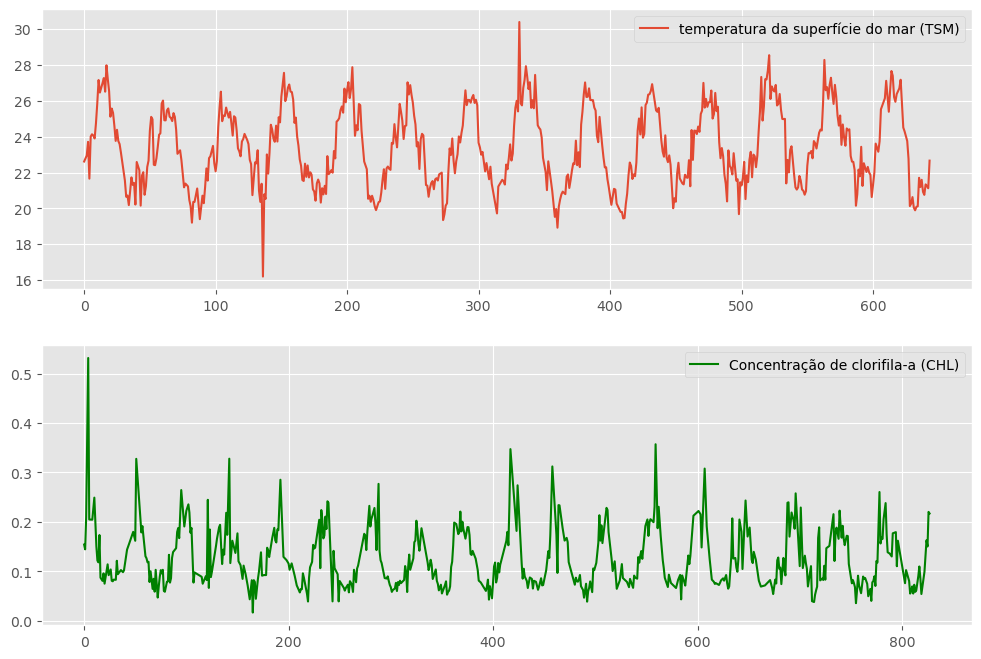
\includegraphics[width=1\linewidth]{lista4-2b]}
	\caption{Séries temporais de TSM e CHL}
	\label{fig:lista4-2b}
\end{figure}
	Analisando visualmente as séries, se nota que existe uma tendência ondulatória na mesma, comparando a tendência das duas, se nota que existe uma diferença de fase entre as duas séries, onde uma depressão de uma representa um pico na outra, a figura \ref{fig:lista4-2c} compara as séries utilizando o mesmo lag no eixo x para as duas, onde esse comportamento fica mais visível.
	
\begin{figure}[H]
	\centering
	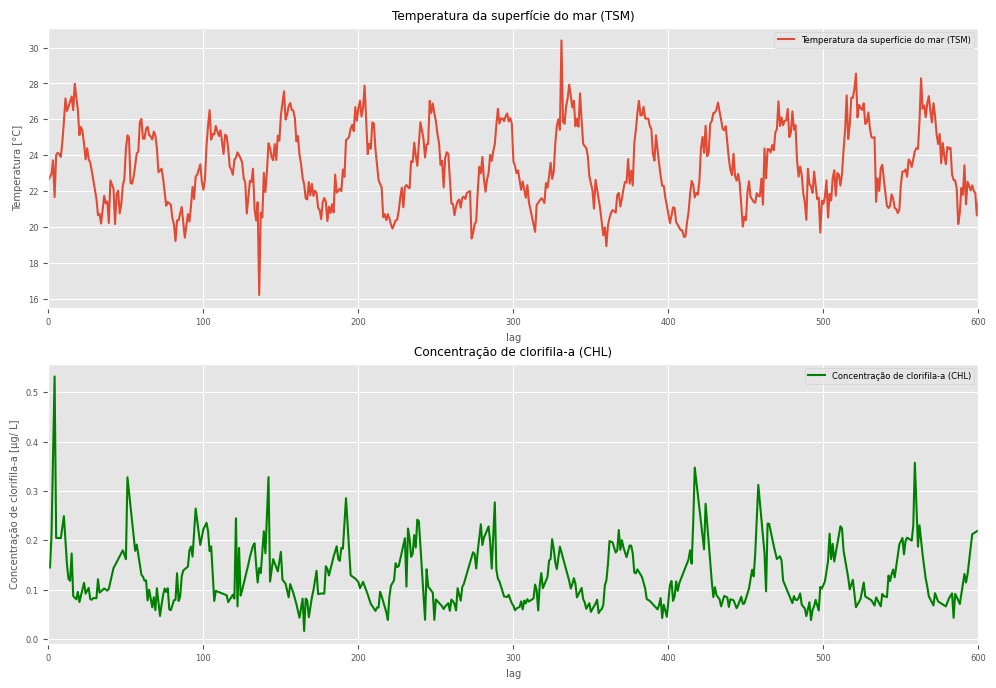
\includegraphics[width=1\linewidth]{lista4-2c}
	\caption{Séries temporais de TSM e CHL com o mesmo tamanho no eixo x}
	\label{fig:lista4-2c}
\end{figure}

Aplicando a função $\log_{10}$ na série de CHL, se obtém a figura \ref{fig:lista4-2d}
\begin{figure}[H]
	\centering
	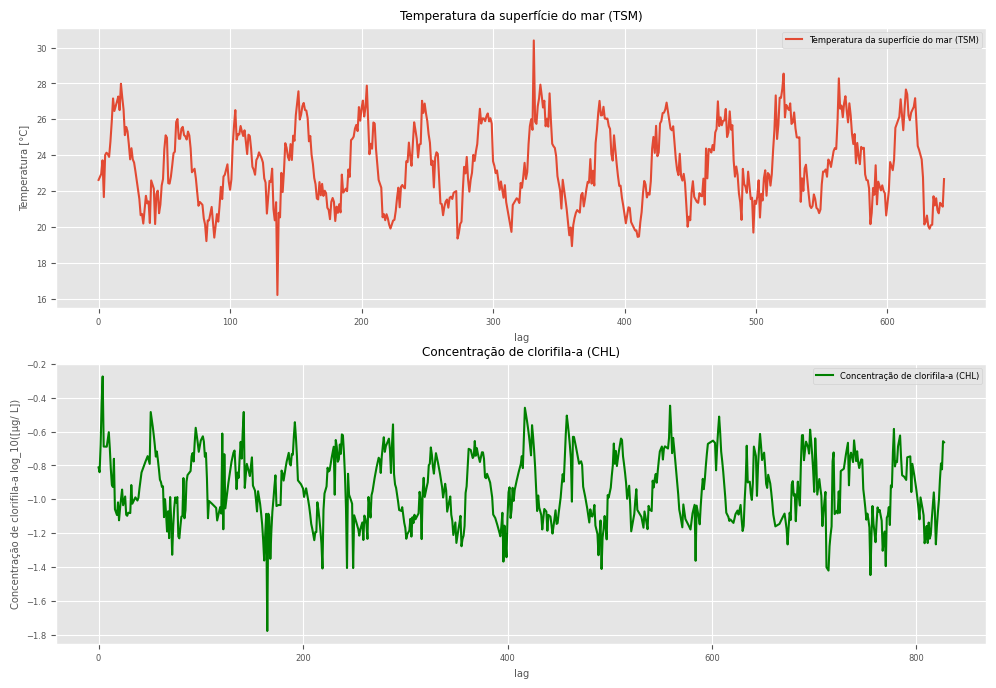
\includegraphics[width=1\linewidth]{lista4-2d}
	\caption{Séries temporais de TSM e de $\log_{10}(CHL)$}
	\label{fig:lista4-2d}
\end{figure}

Removendo a tendência se obtém a figura

\begin{figure}[H]
	\centering
	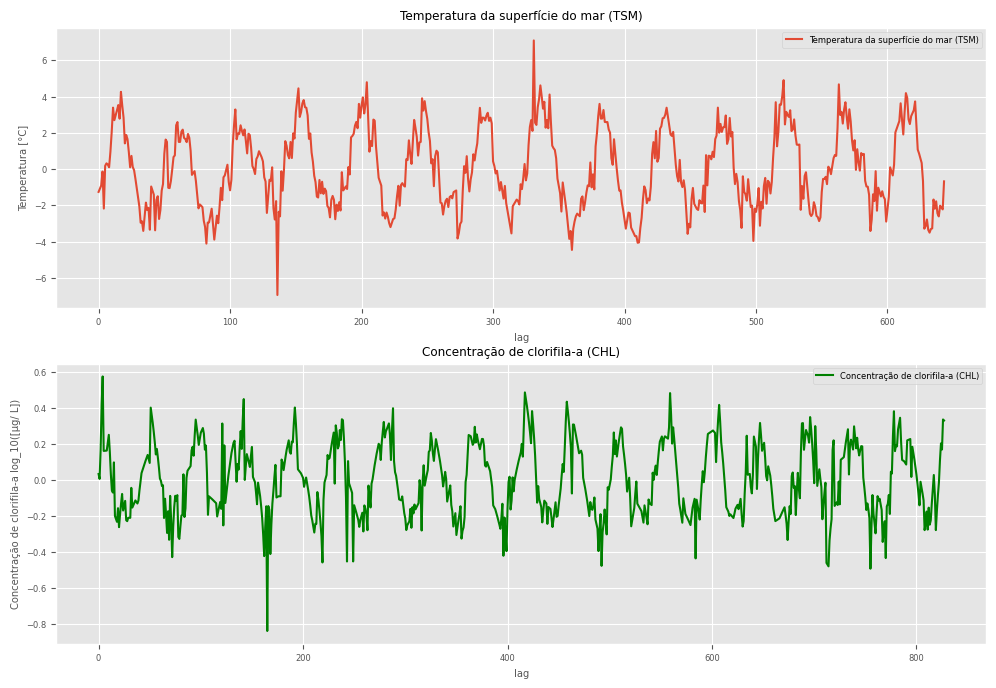
\includegraphics[width=1\linewidth]{lista4-2e}
	\caption{Anomalias nas séries temporais de TSM e de $\log_{10}(CHL)$}
	\label{fig:lista4-2e}
\end{figure}




	
	
\end{document}